\subsection{Skipping Or Changing Coordinates -- Filters}

\begin{pgfplotsxycodekeylist}{\x\ filter,filter point}
The code keys |x filter| and |y filter| allow coordinate filtering which are based on a \emph{single} coordinate. A coordinate filter gets an input coordinate as |#1|, applies some operation and writes the result into the macro |\pgfmathresult|. If |\pgfmathresult| is empty afterwards, the coordinate is discarded. You can also set |\pgfmathresult| to |nan| or |inf| in which case the coordinate can be either discarded (if |unbounded coords=discard| is set) or the plot can be interrupted (the case |unbounded coords=jump|).

The |filter point/.code| filter allows filtering dependent on all components forming a complete point ($x$, $y$ and $z$); it is described below.

It is allowed if filters do not change |\pgfmathresult|. In this case, the unfiltered coordinate will be used.

Coordinate filters are useful in automatic processing system, where \PGFPlots\ is used to display automatically generated plots. You may not want to filter your coordinates by hand, so these options provide a tool to do this automatically.

The following filter adds $0.5$ to every $x$ coordinate.
\begin{codeexample}[]
\begin{tikzpicture}
\begin{axis}[x filter/.code=
	{\pgfmathadd{#1}{0.5}}]
\addplot coordinates {
	(4,0)
	(6,1)
};
\end{axis}
\end{tikzpicture}
\end{codeexample}
Please refer to~\cite[pgfmath manual]{tikz} for details about the math engine of \PGF. Please keep in mind that the math engine works with limited \TeX\ precision.

During evaluation of the filter, the macro |\coordindex| contains the number of the current coordinate (starting with~$0$). Thus, the following filter discards all coordinates after the $5$th and before the $10$th.
\begin{codeexample}[]
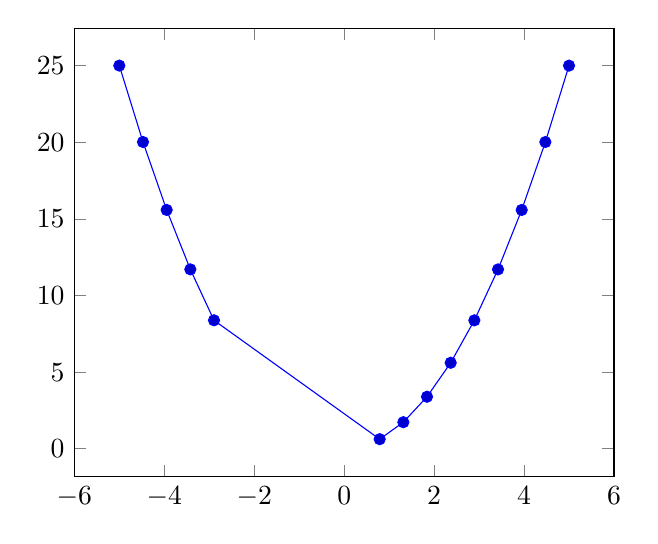
\begin{tikzpicture}
\begin{axis}[
	samples=20,
	x filter/.code={
		\ifnum\coordindex>4
			\ifnum\coordindex<11
				\def\pgfmathresult{}
			\fi
		\fi
	}]
\addplot {x^2};
\end{axis}
\end{tikzpicture}
\end{codeexample}
There is also a style key which simplifies selection by index, see below.

	\PGFPlots\ invokes the filter with argument |#1| set to the input coordinate. For $x$-filters, this is the $x$-coordinate as it is specified to |\addplot|, for $y$-filters it is the $y$-coordinate.

	If the corresponding axis is logarithmic, |#1| is the \emph{logarithm} (see |log basis x| and its variants) of the coordinate as a real number, for example |#1=4.2341|. In case the logarithm was undefined, the argument will be empty.

	The arguments to coordinate filters are minimally preprocessed: first, for logarithmic axes, the \emph{log} of the argument is supplied.  Second, any high level coordinate maps like |x coord trafo| (which may be used to map dates to numbers or string to numbers or so) are applied. In consequence, the |#1| argument is supposed to be a number. No further transformation has been applied.

	Occasionally, it might be handy to get the ``raw'', completely unprocessed input coordinate as it has been reported by the coordinate input routine. This unprocessed data is available in the three math parser constants \declareandlabel{rawx}, \declareandlabel{rawy} and \declareandlabel{rawz} (use \declareandlabel{\pgfmathrawx}, \declareandlabel{\pgfmathrawy} and \declareandlabel{\pgfmathrawz} as a way to assign the value of interest to |\pgfmathresult|). All these values are ready for use in filters (and some other methods influence plots as well).

	If key filters are invoked for |plot table|, access to the current row's data can be achieved using |\thisrow|\marg{column name} (and its variants). This includes all columns of the table.

	The |filter point| key is more technical. It doesn't take an argument: its arguments are given in terms of the |pgfkeys| variables |/data point x|, |/data point y| and |/data point z|. It may change its coordinates using |\pgfkeyssetvalue{/data point x}|\marg{the new value}; access to variables can be get with |\pgfkeysvalueof{/data point/x}| or, if the argument shall be written into a macro, with |\pgfkeysgetvalue|. This filter is evaluated after the other ones.

\end{pgfplotsxycodekeylist}

\begin{stylekey}{/pgfplots/skip coords between index=\marg{begin}\marg{end}}
	A style which appends an |x filter| which discards selected coordinates. The selection is done by index where indexing starts with~$0$, see |\coordindex|. Every coordinate with index $\meta{begin} \le i < \meta{end}$ will be skipped.
\begin{codeexample}[]
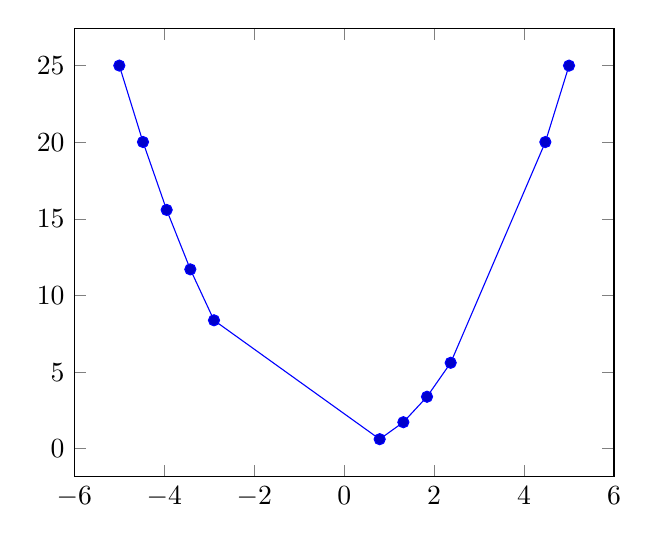
\begin{tikzpicture}
\begin{axis}[
	samples=20,
	skip coords between index={5}{11},
	skip coords between index={15}{18}]

\addplot {x^2};
\end{axis}
\end{tikzpicture}
\end{codeexample}
\end{stylekey}

\begin{pgfplotskey}{each nth point=\marg{integer}}
	A style which appends an |x filter| which discards all but each $n$th input coordinate.
\index{Downsampling}
\end{pgfplotskey}

\begin{pgfplotsxykeylist}{
	restrict \x\space to domain=\meta{min}:\meta{max},
	restrict \x\space to domain*=\meta{min}:\meta{max}}
\label{key:restrict:x:to:domain}
	These keys append $x$ (or $y$ or $z$) coordinate filters to restrict the respective coordinate to a domain. 
	
	The versions without star (like |restrict x to domain|) will assign the value |-inf| if the coordinate is below \meta{min} and |+inf| if the coordinate is above \meta{max}. The starred versions (like |restrict x to domain*|) will truncate coordinates to $[\hbox{\meta{min}}, \hbox{\meta{max}}]$, i.e.\ they assign the value \meta{min} if the coordinate falls outside of the lower limit and \meta{max} if the value falls outside of the upper limit.

	For logarithmic axes, \meta{min} and \meta{max} are \emph{logs} of the respective values.  A variant which uses the non-logarithmic number might be to use |restrict expr to domain={\pgfmathrawx}|\marg{min}\marg{max}.

	The non-starred versions also set |unbounded coords=jump| which leads to interrupted plots.
\begin{codeexample}[]
\begin{tikzpicture}
\begin{axis}[
	restrict y to domain=-10:10,
	samples=1000,
	% some fine tuning for the display:
	width=10cm, height=210pt,
	xmin=-4.7124, xmax=4.7124,
	xtick={-4.7124,-1.5708,...,10},
	xticklabels={$-\frac32 \pi$,$-\pi/2$,$\pi/2$,$\frac32 \pi$},
	axis x line=center,
	axis y line=center]

\addplot[blue] gnuplot[id=tangens,domain=-1.5*pi:1.5*pi] {tan(x)};
\legend{$\tan(x)$}
\end{axis}
\end{tikzpicture}
\end{codeexample}
\end{pgfplotsxykeylist}

\begin{pgfplotskeylist}{%
	restrict expr to domain=\marg{expression}\marg{\meta{min}:\meta{max}},%
	restrict expr to domain*=\marg{expression}\marg{\meta{min}:\meta{max}}%
	}
	Appends an $x$ coordinate filter which sets the $x$ coordinate to |-inf| if the \meta{expression} evaluates to something less than \meta{min} and to |inf| if \meta{expression} evaluates to something larger than \meta{max}.

	The starred variant, |restrict to domain*| assigns \meta{min} if \meta{expression} is less then the lower limit and \meta{max} if it is larger than the upper limit.

	The non-starred version also sets |unbounded coords=jump| which leads to interrupted plots.

	In contrast to |restrict x to domain|, \meta{expression} can depend on anything which is valid during |\addplot|, in particular |\coordindex| or table columns (|\thisrow|\marg{column name} and friends). The expression doesn't need to depend on $x$ at all.
\end{pgfplotskeylist}

\begin{pgfplotskey}{filter discard warning=\mchoice{true,false} (initially true)}
	Issues a notification in your logfile whenever coordinate filters discard coordinates.
\end{pgfplotskey}

